\documentclass[usenames,dvipsnames]{beamer}

\mode<presentation> {
\usetheme{Montpellier}
}

\usepackage{graphicx} % Allows including images
\usepackage{booktabs} % Allows the use of \toprule, \midrule and \bottomrule in tables
\usepackage[frenchb]{babel}
\usepackage[T1]{fontenc}
\usepackage[utf8]{inputenc}
\setcounter{tocdepth}{2}
\graphicspath{{../../Figures/}}

\newcounter{numexos}%Création d'un compteur qui s'appelle numexos
\setcounter{numexos}{0}%initialisation du compteur
\newcommand{\exercice}[1]{%Création d'une macro ayant un paramètre
\addtocounter{numexos}{1}%chaque fois que cette macro est appelée, elle ajoute 1 au compteur numexos
\textcolor{DarkOrchid}{Exercice\,\thenumexos\,:}\,#1%Met en rouge Exercice et la valeur du compteur appelée par \thenumeexos
}

\setbeamertemplate{title page}{
    \centering

    \huge\bfseries
    Machine Learning Tek 5

\begin{figure}[!h]

\includegraphics[width=8cm]{knn_k=20_samples=100000_sigma=1}
\end{figure}

    }

\title[FTML]{title}


\date{} % Date, can be changed to a custom date

\makeatletter
\let\@@magyar@captionfix\relax
\makeatother

\begin{document}

\begin{frame}
\titlepage % Print the title page as the first slide
\end{frame}

\section{Textbooks}

\begin{frame}{Textbooks}

Textbooks are better than slides !

\url{https://github.com/nlehir/ML_tek5/blob/main/references.pdf} 

\end{frame}

\begin{frame}{FTML}

    I also make a course at Epita, you can find some material there and many practical sessions

    \url{https://github.com/nlehir/FTML} 

\end{frame}

\section{Introduction to AI and ML}

\begin{frame}{Definitions}

    We will start by the a short general discussion on \textbf{{AI and ML}}.

    Quick remarks:
    \begin{itemize}
	\item Machine learning (ML) is \textbf{{easier}} to define than AI. Several
    definitions of AI exists, and the term can be used in different contexts. However the practical usage of the term "ML" has been shifting a bit for the last few years.
	\item These topics are evolving at a fast pace, it is hard to be up to date on everything !
    \end{itemize}
\end{frame}


\begin{frame}
\frametitle{Example 1: digit classification}
\begin{figure}[!h]
\centering
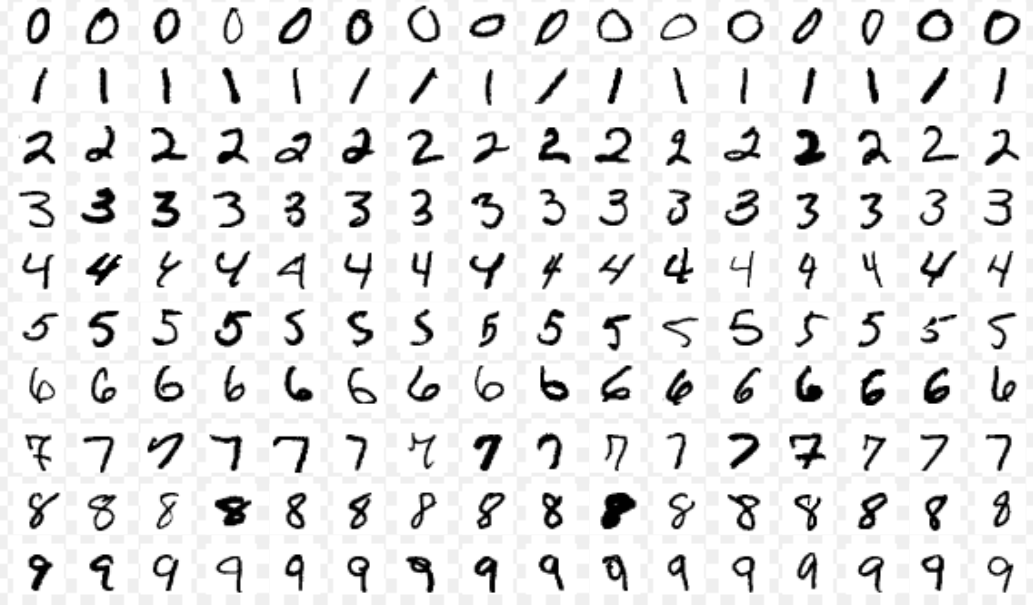
\includegraphics[width=8cm]{mnist.png}
\caption{MNIST database \cite{lecun-mnisthandwrittendigit-2010}}
\label{mnist}
\end{figure}
\end{frame}

\begin{frame}
\frametitle{Example 2: robots}
\begin{itemize}
	\item Boston Dynamics robots (video)
    \item \url{https://www.youtube.com/watch?v=LikxFZZO2sk}
    \item \url{https://www.youtube.com/watch?v=g0TaYhjpOfo}
    \item \url{https://www.youtube.com/watch?v=tF4DML7FIWk&t=57s} 
    \item \url{https://www.youtube.com/watch?v=EezdinoG4mk} 
\end{itemize}
\end{frame}

\begin{frame}
\frametitle{Example 3: go player}
\begin{figure}[!h]
\centering
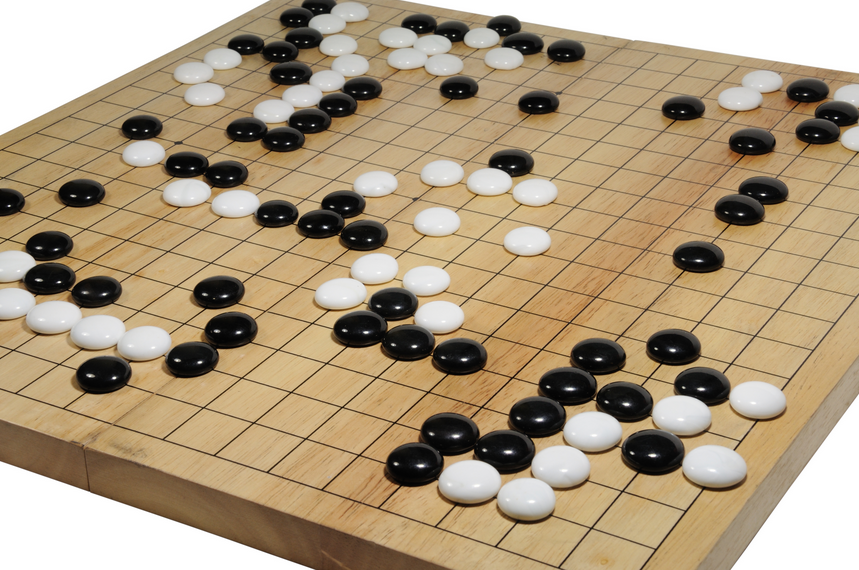
\includegraphics[width=8cm]{go.png}
\caption{Go game, won by AlphaGo in 2017 \cite{SilverHuangEtAl16nature}}
\label{mnist}
\end{figure}
\end{frame}


\begin{frame}{Example 4: audio engineering helper}

    \begin{figure}[htpb]
    	\centering
    	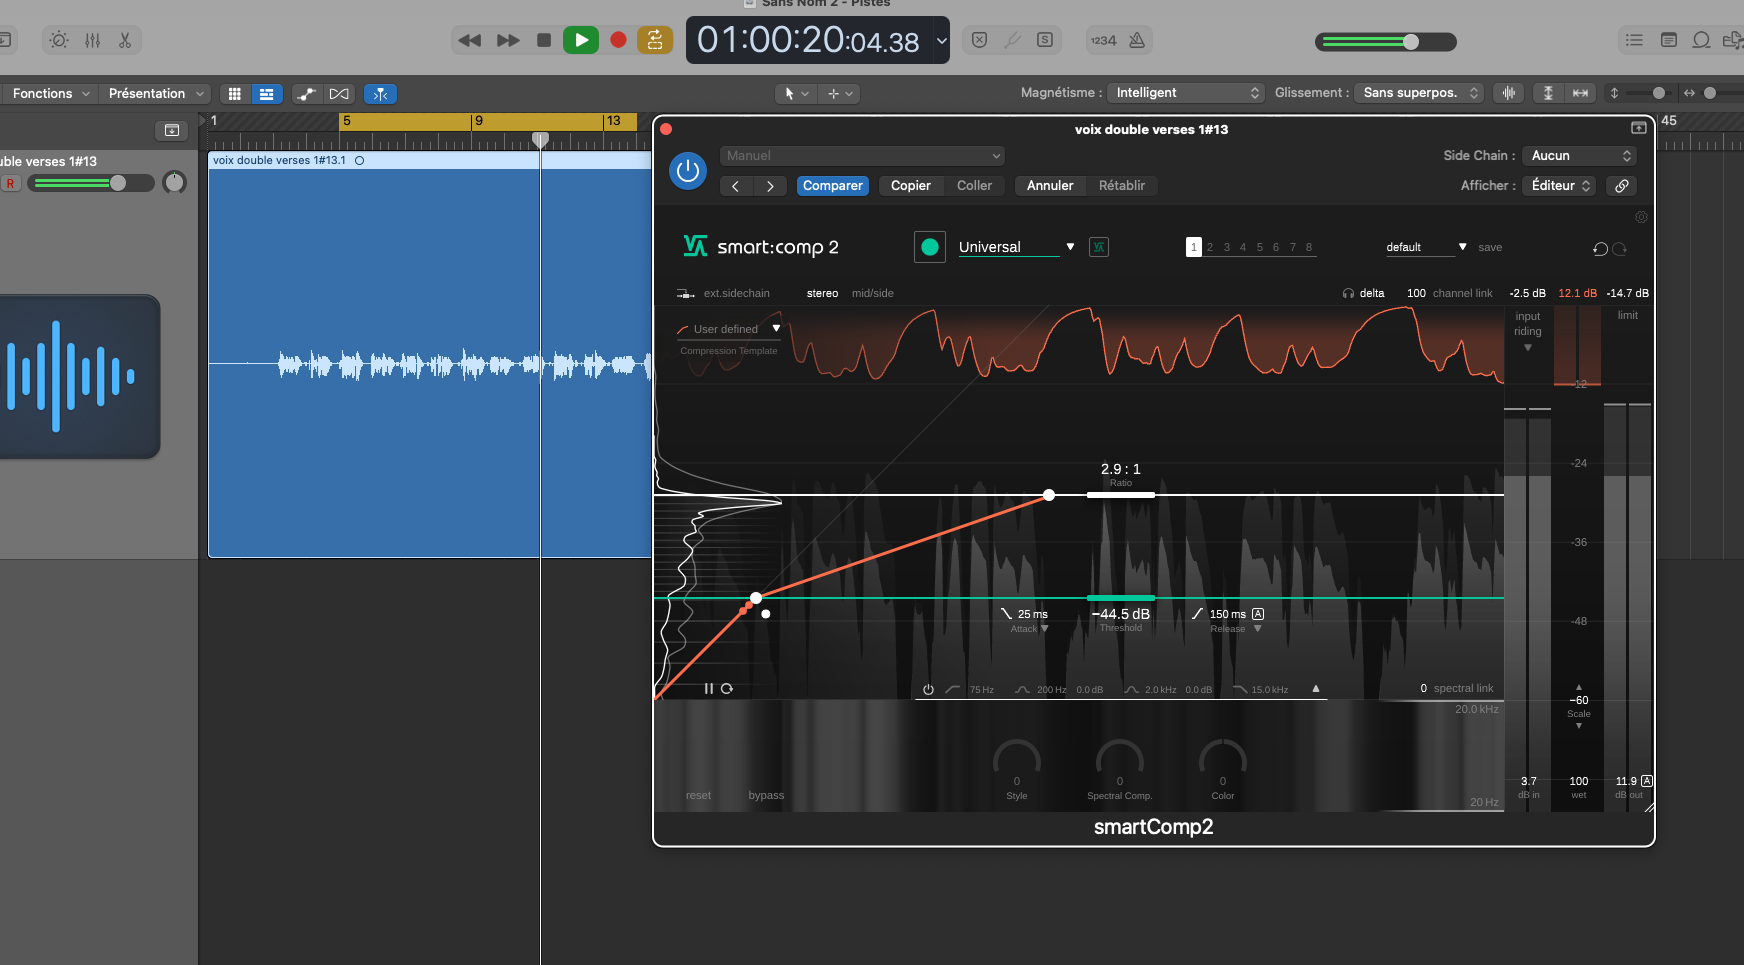
\includegraphics[width=0.8\textwidth]{smartcomp}
    	\caption{Semi-automatic compressor: \url{https://www.sonible.com/smartcomp2/}}
    	\label{fig:Semi-automatic-comp}
    \end{figure}

\end{frame}

\begin{frame}{Example 5: coffee machine}
    \begin{figure}[htpb]
        \centering
        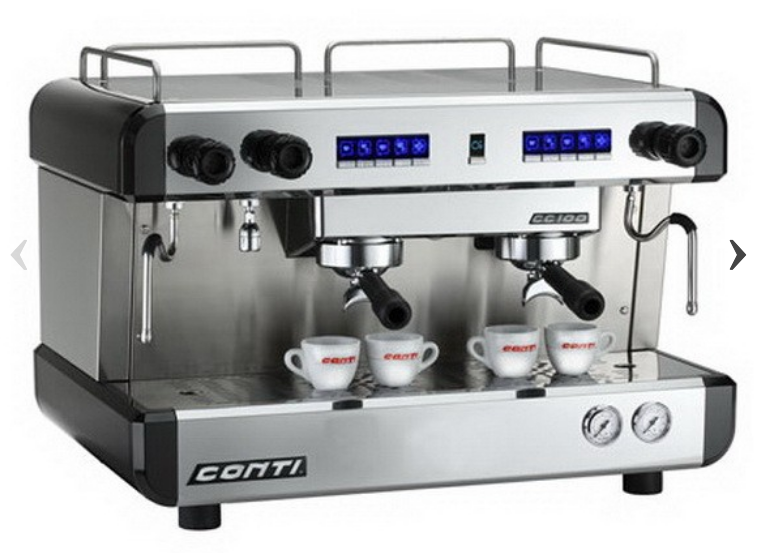
\includegraphics[width=0.6\linewidth]{cafe}
	\caption{Coffee machine (\scriptsize{https://www.stockresto.com/fr/machine-a-cafe/83-machine-a-cafe-conti-cc100-2-groupes.html})} 
    \end{figure}
\end{frame}

\begin{frame}
\frametitle{Introduction examples}
\begin{itemize}
	\item 
	\begin{itemize}
		\item Boston Dynamics robot
		\item MINST classification
		\item AlphaGo
		\item AI compressor
		\item Coffee Machine
\end{itemize}
    \item All of them perform different tasks but could be qualified as "AI" (or are branded as AI) ?
\end{itemize}
\end{frame}

\begin{frame}{Definition}
   \begin{itemize}
       \item Example definition of AI : "the theory and techniques aiming at emulating intelligence".
       \item Hence defining AI requires definining "intelligence".
   \end{itemize}
\end{frame}

\begin{frame}{Turing test}
    \begin{itemize}
	\item It is reasonable to say that the problem of AI was born at the same
        time as that of \textbf{{Computer Science}}. One of the founders of
            Computer Science is Alan Turing (1912-1954). 
        \item In 1950, with the article \textbf{{"Computing machinery and intelligence"}} \cite{Turing2009}, Turing introduces the \textbf{{Turing test}}. 
	\item One of the forms of a Turing Test is a game in which a computer tries to behave like a human by answering questions.
    \end{itemize}
\end{frame}


\begin{frame}
   \begin{figure}[htpb]
       \centering
       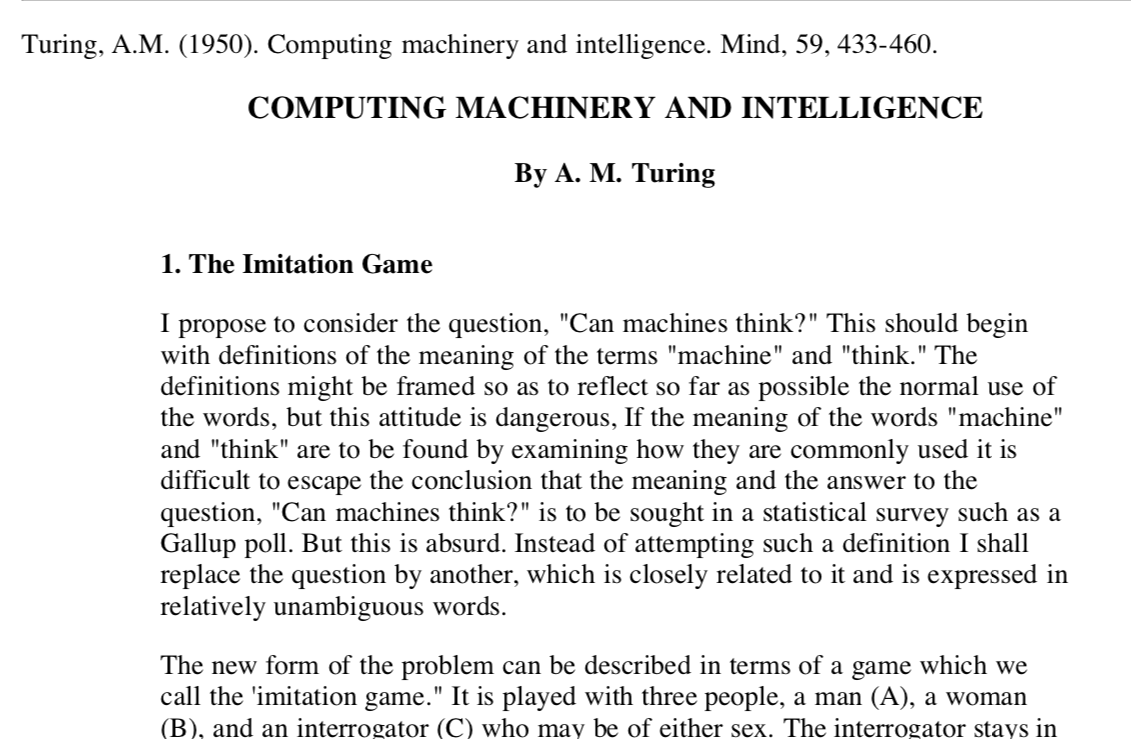
\includegraphics[width=0.8\linewidth]{turing}
       \label{fig:turing}
   \end{figure} 
\end{frame}

\begin{frame}{Turing test}
    \begin{itemize}
        \item Importantly, Turing stresses that the terms "think", and "machines" are far from being \textbf{{unambiguous}}. 
	\item Many (most ?) questions regarding our own "intelligence" and "consciousness" as humans remain open today.
	\item In that respect, it is tricky to give a indisputable definition of AI.
    \end{itemize}
\end{frame}


\begin{frame}{Moravec Paradox}
   \begin{itemize}
       \item It is harder to emulate or simulate simple sensorimotor capacities than level abstract reasoning.
       \item ie : the sensorimotor system of an ant is harder for us to emulate than beating the world champion at chess (Deep Blue, 1997).
   \end{itemize} 
\end{frame}

\begin{frame}{Strong AI, Weak AI}
   \begin{itemize}
       \item There exists a distinction between \textbf{{Weak AI}}, and a \textbf{{hypothetical}} AI called \textbf{{Strong AI}}. 
       \item \textbf{{Weak AI}} (also known as \textbf{{narrow AI}}) designed and trained for a particular task (e.g. Siri).
       \item \textbf{{Strong AI}} (also known as Artificial General
           Intelligence AGI) : able to find a solution, faced with an
           \textbf{{unfamiliar task}}. This is slightly ill-defined.

	   \textbf{However} other people probably see the current state of LLMs as a form of AGI. But again, this depends on how these concepts are defined.
   \end{itemize} 
\end{frame}

\begin{frame}{Conscious reasoning}
    Broadly speaking, the first phases of research in AI were more dedicated to
    emulating the \textbf{{conscious brain.}} 
    \begin{itemize}
        \item logic programming (Prolog)
        \item expert systems
    \end{itemize}
\end{frame}

\begin{frame}{History : AI Winter (1970's)}
   \begin{itemize}
       \item In 1974 fundings for AI reseach started being cut by goverments because of unsuccessful projects.
        \item there were actually several so-called "AI winters".
   \end{itemize}
\end{frame}

\begin{frame}{Famous AI : Deep Blue (1997)}
   \begin{itemize}
       \item Beat the world chess champion Gary Kasparov in 1997.
           \item 
               \begin{figure}[htpb]
                   \centering
                   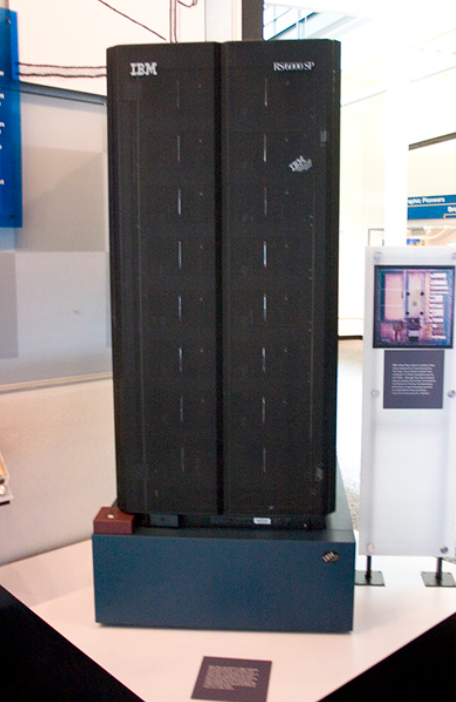
\includegraphics[width=0.3\linewidth]{blue}
                   \label{fig:blue}
		   \caption{{Deep Blue}}
               \end{figure}
            \item Despite its name, Deep Blue is \textbf{{not related}} to Deep
                learning !
   \end{itemize} 
\end{frame}

\begin{frame}{Decision trees and limitations}
    One of the underlying mechanisms of Deep Blue were \textbf{{Decision
    Trees}} / minimax algorithm.
    \begin{itemize}
	\item Let $p$ be the \textbf{{branching factor}} of the tree. (Here, the average number of children at each node)
	\item Let $d$ be the \textbf{{depth}} of the tree. 
	\item What is the order of magnitude of the number of nodes in the tree ?
    \end{itemize}
\end{frame}


\begin{frame}{Limitations of the method}
    \begin{itemize}
	\item Let $p$ be the \textbf{{branching factor}} of the tree of actions. (Here, the average number of children at each node)
	\item Let $d$ be the \textbf{{depth}} of the tree. 
	\item What is the order of magnitude of the number of nodes in the tree ?
	\item So in order to run the minimax algorithm needs to perform $\mathcal{O}(p^d)$ evaluations.
    \end{itemize}
\end{frame}

\begin{frame}{Exercise}
    \exercice{\textbf{Computation time}}
    \begin{itemize}
        \item In the \textbf{{Othello game}}, the average number of actions in each state is around $8$.
	\item We assume that the evaluation for one leaf node takes $1\times 10^{-6}$ seconds.
	\item How long would be the search of the minimax if we look \textbf{{$10$}}  actions ahead ?
	    \item
		\begin{figure}
	    \begin{center}
		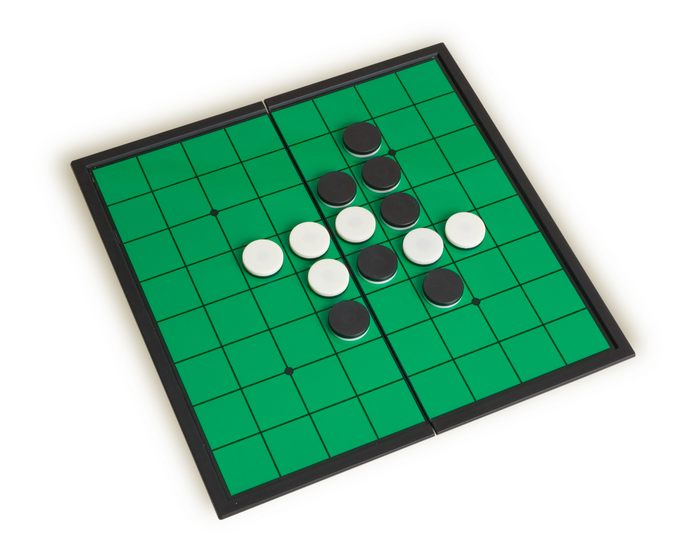
\includegraphics[width=4.5cm]{othello.png}
	    \end{center}
	    \label{fig:label}
	    \end{figure}
    \end{itemize}
\end{frame}


\begin{frame}{Exercise}
    \begin{itemize}
        \item In the \textbf{{Othello game}}, the average number of actions in each state is around $8$.
	\item This duration is too large for practical applications.
	    \item
		\begin{figure}
	    \begin{center}
		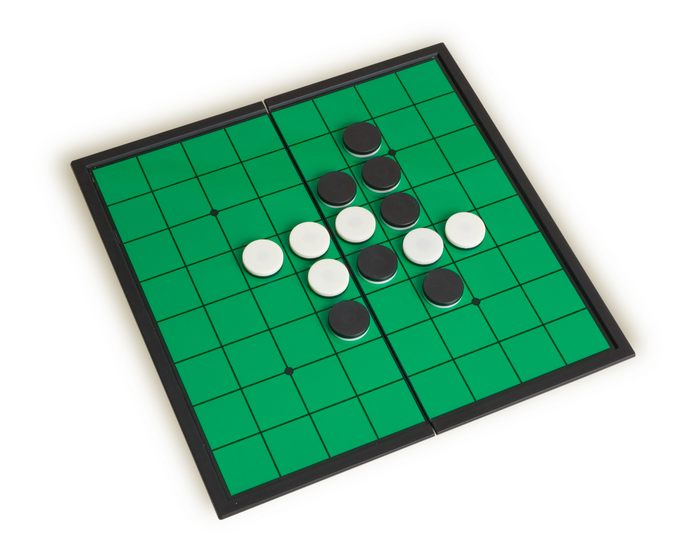
\includegraphics[width=4.5cm]{othello}
	    \end{center}
	    \label{fig:label}
	    \end{figure}
    \item In AlphaGo, the algorithm used was really different (Deep Reinforcement Learning.)
    \end{itemize}
\end{frame}

\begin{frame}{2000's and 2010's}
    \begin{itemize}
        \item Around the 2000's, there has been a shift in the focus of AI.
        \item Machine learning and data science have become prominent research and industrial topics.
        \item We could argue that emulating the \textbf{{unconscious brain}} is
            more of a focus today.
        \item An important contemporary and future trend in research might be
            to connect research on emulating the conscious brain and research
            emulating the unconscious brain.
    \end{itemize}
\end{frame}

\begin{frame}{Interesting slides on AI history}

    \url{https://home.mis.u-picardie.fr/~furst/IA.php} 

\end{frame}

\begin{frame}{Machine learning: proposition of definitions}
    \begin{itemize}
        \item (proposed definition of) \textbf{learning}: "Modification of a behavior, based on a life experiment"
        \item \textbf{{Machine learning}}: "artificial intelligence which can learn
    and model some phenomena without being explicitely programmed".
        \item In Machine learning, some parameters are learned in an
            \textbf{semi-automatic way}, based on a \textbf{dataset} in order to solve a problem or to optimize a
            solution.
    \end{itemize}
\end{frame}

\begin{frame}{Classical programming vs ML}
    \begin{itemize}
	\item Classical program: predict the total amount of money spent, based on the number of fruits bought and the price of each individual fruit (a summation is enough)
	\item ML program: predict which fruit a person buys, based on a database of customers and on some information about this person (e.g. buying log, age, profession).
    \end{itemize}
\end{frame}

\begin{frame}{Use cases of ML}
    ML is useful for problems:
\begin{itemize}
    \item that we cannot solve direcly thanks to an explicit representation (such as the amount of money spent in the previous first example).
    \item that we could solve explicitely, but the computationnal ressources would be too heavy (e.g. molecular dynamics), so we \textbf{approximate} a solution with ML.
\end{itemize}

    Sometimes, ML solutions to a problem are effective, but the underlying mechanism is not perfectly understood (like in deep learning).
\end{frame}

\begin{frame}{Denomination}
    \begin{itemize}
    	\item The name "machine learning" is rather deceitful !
	\item It is no more machine driven than any algorithm or coffee machine.
	\item The denomination "statistical learning" is used in some contexts.
    \end{itemize}
\end{frame}

\begin{frame}{Machine learning}
   Machine learning has received attention and funding because it has reached
    state-of-the-art efficiency on several problems such as:
    \begin{itemize}
        \item computer vision
        \item spam classification
        \item machine translation
        \item speech recognition
        \item self-driving cars
	\item text, image, music generation
    \end{itemize}
    \textbf{{Deep learning}} is involved in all these state-of-the-art solutions.
\end{frame}

\begin{frame}{Example 1: ImageNet}
    \begin{itemize}
        \item A database of images (more than $15$M), hand-annotated in order to
            indicate what objects are present in the image. More than $20000$
            categories of images.
        \item Contest: ImageNet Large Scale Visual Recognition Challenge.
        \item The best classification (top-5 error rate) went from $25\%$ in 2011 to
            $\simeq 15.3\%$ in 2012.
        \item The technology used was deep learning, exploiting GPUs (AlexNet).
    \end{itemize}

    \url{https://paperswithcode.com/sota/image-classification-on-imagenet} 
\end{frame}

\begin{frame}{Example 2: AlphaGo}
   \begin{itemize}
       \item In 2015: beats a professionnal player. In 2017: beats the world
           champion.
        \item Uses several technologies: among them \textbf{{Deep reinforcement
            learning.}} 
        \item Improvements: AlphaGo Zero, trained without a database of played
            games. In 2017, AlphaZero beats AlphaGo Zero after $3$ days of
            learning.
   \end{itemize} 
\end{frame}

\begin{frame}{Example 3: AlphaFold}
    \begin{itemize}
        \item Goal: to predict the spatial configuration of proteins, from
            their DNA sequence.
        \item Achieves a breakthgough performance on the CASP challenge:
            \begin{itemize}
                \item 2018: more than $50\%$ GDT (Global distance test),
                    whereas it was $\leq 40\%$ before then.
                \item 2020: $92,4\%$ GDT. At a $\geq 90\%$ score, the method is
                    considered competitive with experimental methods..
            \end{itemize}
        \item \url{https://alphafold.ebi.ac.uk/} 
        \item Also based on Deep learning.
    \end{itemize}
\end{frame}

\begin{frame}{Deep learning $\subset$ Machine Learning $\subset$ AI}

	\begin{itemize}
		\item Machine learning is not only about deep learning.
		\item Some chapters of the course will be dedicated to neural networks and deep learning, as it is a really important contemporary topic. But we will not focus only on deep learning, but rather on more elementary / fundamental tools. 
		\item Globally speaking, ML has a strong \textbf{experimental} component in industrial applications.
	\end{itemize}
\end{frame}

\begin{frame}
\frametitle{AI and Machine Learning}
In the four first examples, according to you which one are NOT a Machine Learning system ?
\end{frame}

\begin{frame}
\frametitle{AI and Machine Learning}
\begin{itemize}
	\item Alpha Go : Machine Learning (Reinforcement Learning)
	\item MNIST : Machine Learning (Supervised Learning)
	\item Coffee Machine : no Machine Learning (Automation)
	\item Boston Dynamics : no Machine Learning (Robotics)
	\item \textbf{{edit : }} while the robots on the video have no Machine Learning, Boston Dynamics seems to now show interest in the topic. ML technologies might start being implemented in their robots, especially for artificial vision.
\end{itemize}
\end{frame}

\begin{frame}{ML revolution}
\begin{itemize}
    \item Technical progress in the computing and storage capacities
    \item Increase in amount of \textbf{available data}. According to IBM, $10^{18}$
        bytes are created each day.
    \item Progress in algorithmic methods to analyze the data.
\end{itemize}
    
\end{frame}

\begin{frame}{ML revolution II}

    \begin{itemize}
	\item The speed of evolution has increased again with LLMs (first Chat GPT release: 2022)
	\item Spectrum of activities between maths and computer science: the jobs linked to AI and ML evolve. We could argue that the balance is more shifted towards data engineering / devops / mlops / computer science in general
	    than 20 years ago.
	\item In this course, we will mention LLMs, but we will not go in depth on the topic (also: I am not an LLM expert).
    \end{itemize}

\end{frame}

\section{Learning paradigms}
\frame{\tableofcontents[currentsection]}

\subsection{Supervised learning}%
\label{sub:supervised_learning}

\begin{frame}{Supervised learning}

    Predict an output from an input.
    \begin{itemize}
    	\item discrete output: classification
	\item continuous output: regression
    \end{itemize}

    We learn from a dataset $D_n$ of $n$ \textbf{labeled examples}; 
\begin{equation}
    D_n =\{(x_i,y_i), i\in[1, n]\}
\end{equation}

    Do not hesitate to ask for a clarification when a notation is unclear.
\end{frame}

\begin{frame}{Supervised Learning: example of regression}
        \begin{itemize}
            \item $x$: age and height of a person. 
                Here $x$, is a \textbf{{vector}} containing $2$ \textbf{{features}}.
            \item $y$:  record on a $100$ meters track
        \end{itemize}
\end{frame}

\begin{frame}{Regression: raw inputs}
       \begin{tabular}{cl}  
         \begin{tabular}{c}
           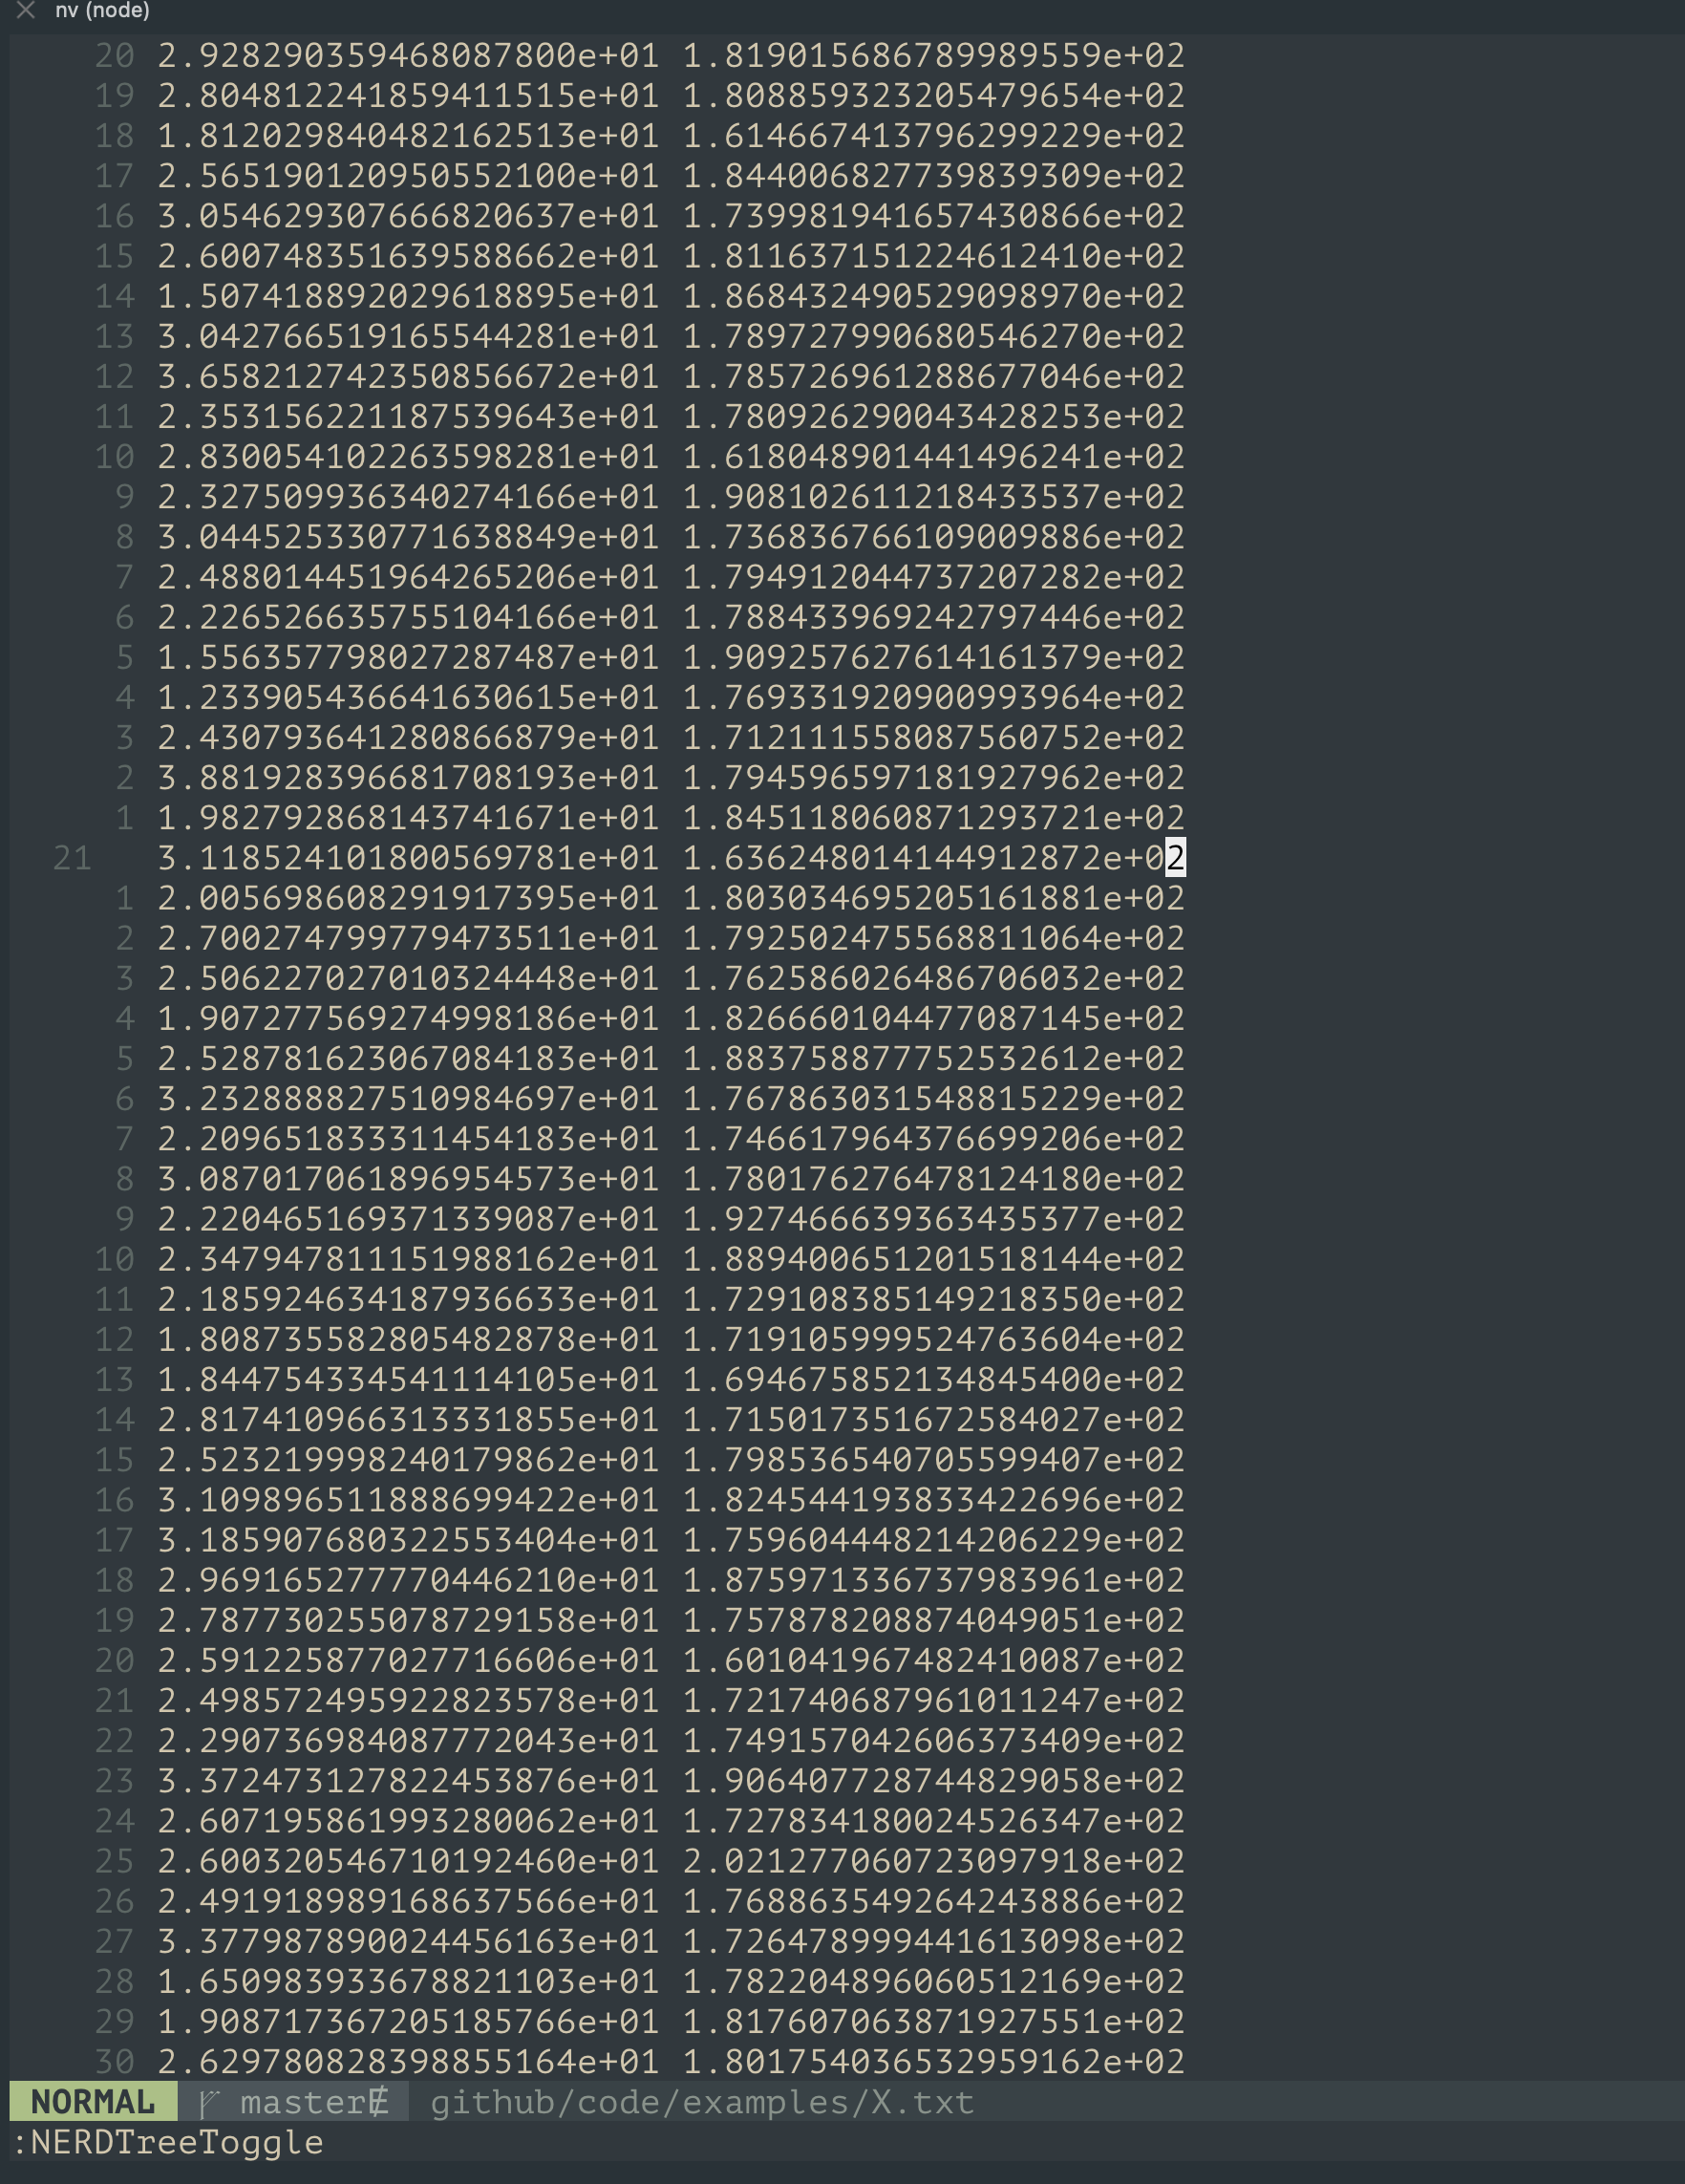
\includegraphics[width=5.2cm]{X}
           \end{tabular}
           & \begin{tabular}{l}
             \parbox{0.5\linewidth}{%  change the parbox width as appropiate
Input data.
    }
         \end{tabular}  \\
\end{tabular}
\end{frame}

\begin{frame}{Regression: raw ouptuts}
       \begin{tabular}{cl}  
         \begin{tabular}{c}
           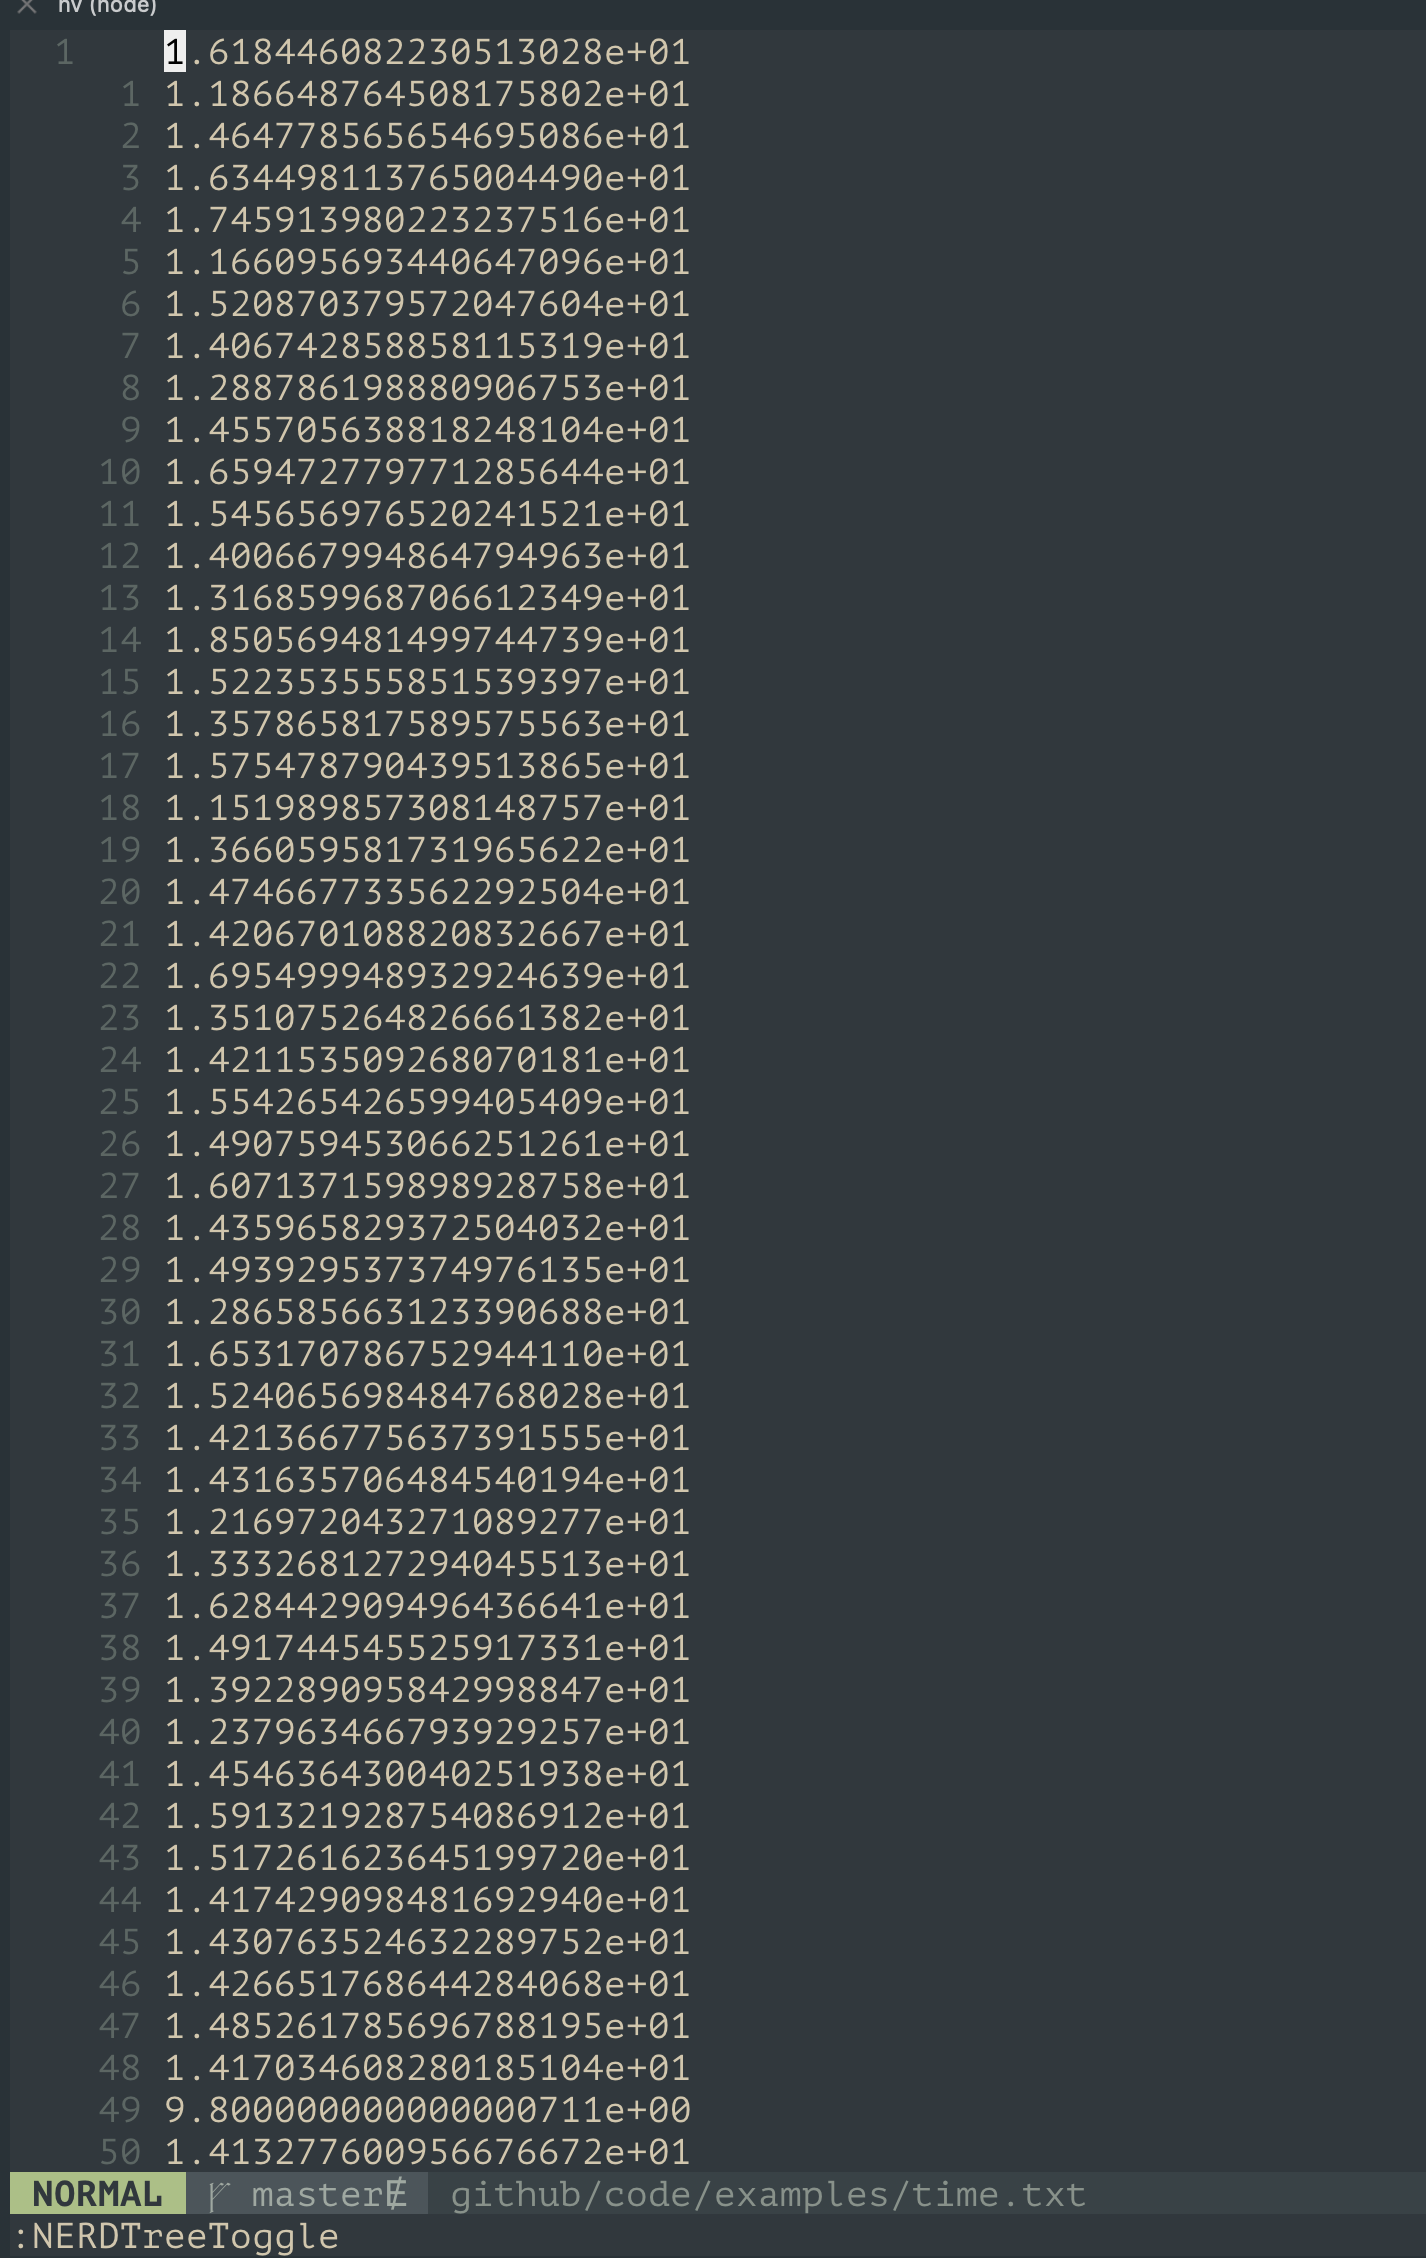
\includegraphics[width=4.2cm]{time}
           \end{tabular}
           & \begin{tabular}{l}
             \parbox{0.5\linewidth}{%  change the parbox width as appropiate
    \exercice{}
    \addtocounter{numexos}{-1}

    Our objective is to build  a function that predicts the output (100 meters track record) as a function of the \textbf{input} (height and age of the person).

    What order of magnitude of precision do we expect to obtain with this example ?

    }
         \end{tabular}  \\
\end{tabular}
\end{frame}

\begin{frame}{Random variables}

    In a machine learning problem, there is (almost) always a statistical error associated with a prediction. Our goal is to minimize it !
    \\

    Datasets should be seen as \textbf{sampled from a random variable}. Hence, \textbf{any quantity derived from the dataset} should be analyzed as a random variable as well.
\end{frame}


\subsection{Unsupervised learning} % (fold)
\label{sub:unsupervised_learning}

\begin{frame}
\frametitle{Unsupervised Learning}
\begin{itemize}
	\item From a number of samples ${x_i}$, we want to retrieve information on
        their structure: \textbf{{modelisation}}.
    \item
        \begin{itemize}
        \item density estimation
        \item clustering
        \item dimensionality reduction
    \end{itemize}
\end{itemize}
\end{frame}


\begin{frame}
\frametitle{Density estimation}
\begin{itemize}
    \item density estimation: anaylze the distribution of the data.
\begin{figure}[htpb]
    \centering
    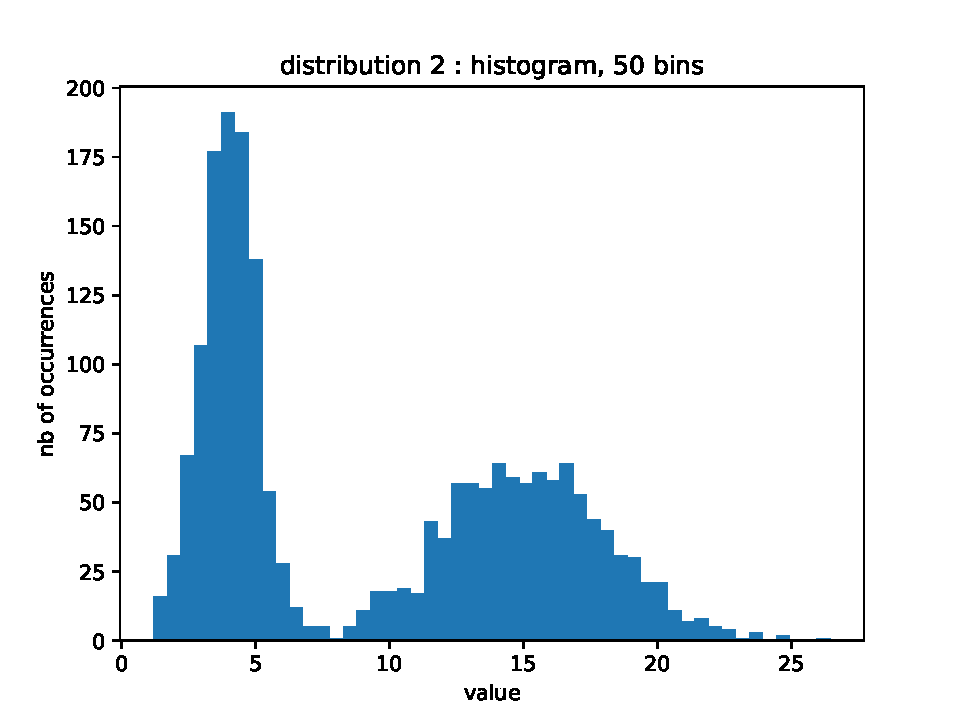
\includegraphics[width=0.5\linewidth]{bimodal}
    \caption{Histogram of random data}
    \label{fig:bimodal}
\end{figure}
\end{itemize}
\end{frame}


\begin{frame}{Clustering}
\begin{figure}[htpb]
	\centering
	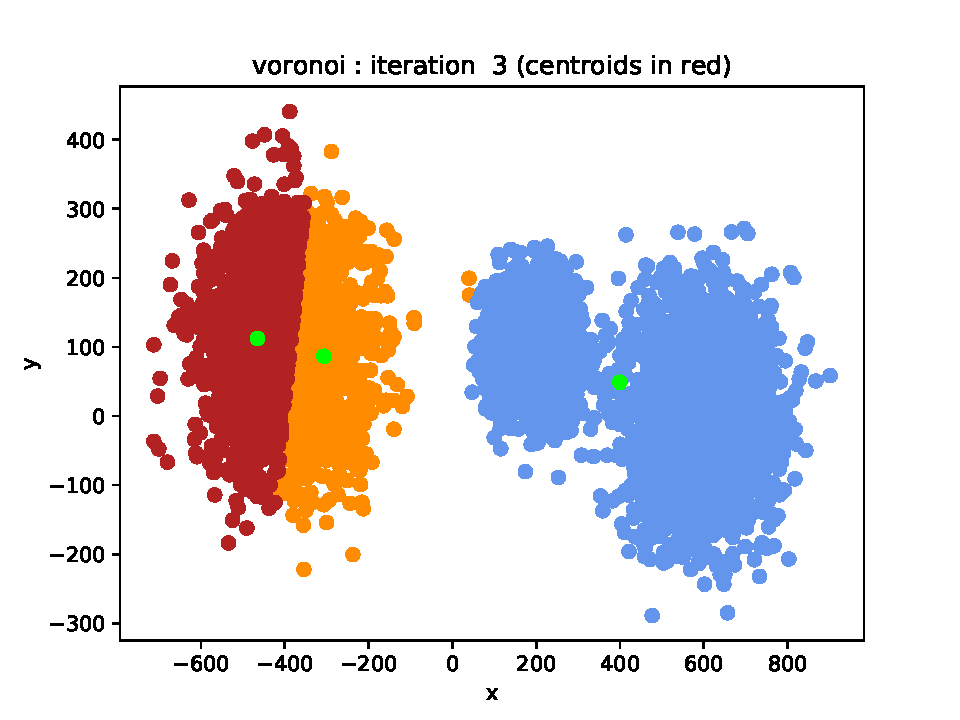
\includegraphics[width=0.7\textwidth]{it_3_assign_voronoi}
	\caption{K-means clustering}
	\label{fig:if_3_assign_voronoi}
\end{figure}
\end{frame}

\begin{frame}{Dimensionality reduction}
\begin{figure}[htpb]
	\centering
	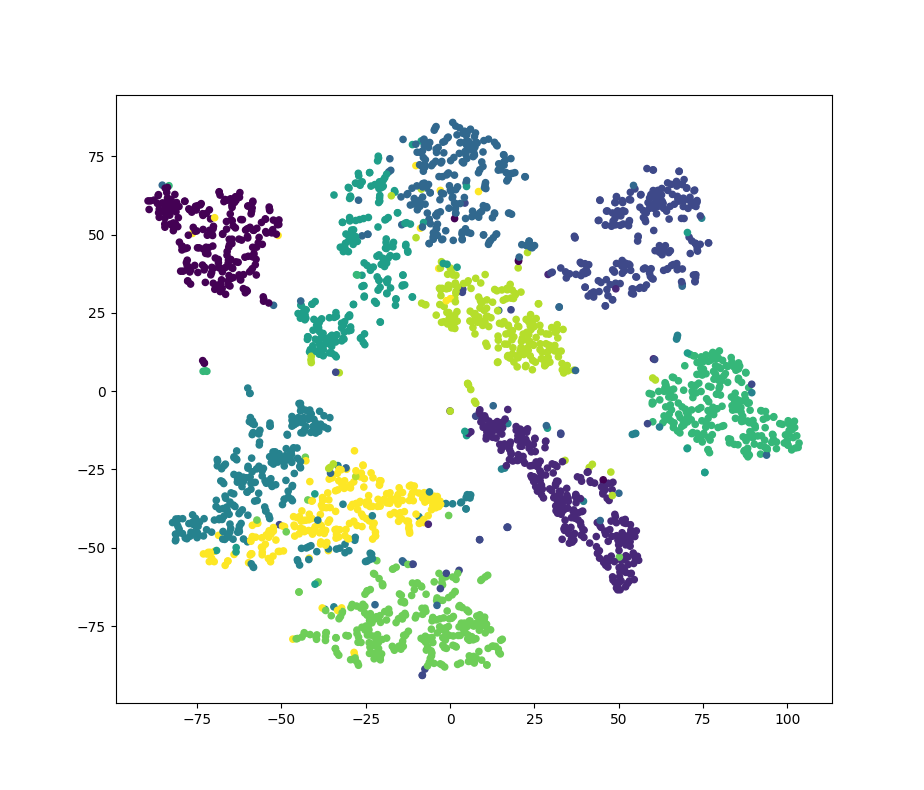
\includegraphics[width=0.65\textwidth]{tsne}
	\caption{t-SNE projection of the MNIST dataset.}
	\label{fig:}
\end{figure}
\end{frame}

\subsection{Reinforcement learning} % (fold)
\label{sub:reinforcement_learning}

\begin{frame}
\frametitle{Reinforcement Learning}
\begin{itemize}
	\item A \textbf{more general paradigm} that describes an \textbf{agent} in a \textbf{world}.
	\item The standard formalization was the one proposed by Richard Sutton \cite{Sutton1998}.
	\item At each time, the world is in a state $s$. An agent perfoms an \textbf{action} $a$ according to a \textbf{policy} $\pi$. When performing an action, the agent receives an \textbf{reward} $r$.
\end{itemize}
\end{frame}

\begin{frame}{Reinforcement Learning applications}
    \begin{itemize}
	\item	Example : some Chessplayers, AlphaGo, automatic vacuum cleaner,
        self-driving cars (trajectory optimization, parking, etc.)

    \item    healthcare: \url{https://arxiv.org/pdf/1908.08796.pdf} 
        \item \url{https://deepmind.com/blog/article/alphago-zero-starting-scratch} 

    \end{itemize}
    
\end{frame}

\begin{frame}
\frametitle{Reinforcement Learning}
\begin{itemize}
	\item At each time, the world is in a state $s$. An agent perfoms an \textbf{action} $a$ according to a \textbf{policy} $\pi$. When performing an action, the agent receives an \textbf{reward} $r$.
	\item The agent wants to learn an \textbf{optimal policy}, meaning the policy that maximises its reward (or rather the \textbf{aggregation} of rewards).
\end{itemize}
\end{frame}

\begin{frame}
\frametitle{This paradigm has many variants}
\begin{itemize}
	\item 	State $s$, action $a$, policy $\pi$, reward $r$.
	\item	Is the policy \textbf{deterministic }? Is it \textbf{stochastic } ? 
	\item	Does the agent have a \textbf{model} of its environment ? 
	\item	How many steps ahead should the agent look ? 
	\item	All these conditions change the way the problem should be addressed and solved.
\end{itemize}
\end{frame}

\begin{frame}
\begin{itemize}
	\item These paradigms can be mixed. For instance,
	\begin{itemize}
		\item unsupervised learning can be used in a supervised learning problem (semi-supervised learning)
		\item unsupervised learning and supervised learning can be used in a reinforcement learning problem
		\item \textbf{self-supervised learning} creates labels from the dataset itsself. 
	\end{itemize}
	\item Given a problem and a dataset, formalizing a problem as a supervised learning or unsupervised learning task is a \textbf{choice}.
	\item Often, obtaining labels for all samples is a hard, long, or even impossible process: e.g. labelling millions of images. Importantly, the dataset collection, preparation or preprocessing is at least as important as the algorithms that are run on it !
\end{itemize}
\end{frame}

\subsection{Examples}%
\label{sub:examples}

\begin{frame}{Example I: what type of learning is it ?}

    Predict the winning team of an NBA game at half-time.
\begin{itemize}
    \item Dataset: $15$ years of games (comments, text): approximately $17000$
        games.
    \item The dataset is preprocessed to have as an input a time-series: each
        time contains the score \textbf{{and}}  $10$ technical features (rebounds, etc.).
        So for each time the dimension is $11$. Each game is a matrix of size $
        1440\times 11$, reorganized as a line vector.
    \item Output: Receiving team wins or looses
    \item Evaluation metric: "0-1" loss ($1$ if error, $0$ otherwise)
\end{itemize}
    
\end{frame}

\begin{frame}{Example II: what type of learning is it ?}
    Predict the quantity of oil in a rock.
    \begin{itemize}
        \item Input: tomographic image of a rock.
        \item Output: material of the rock, average presence of residual oil in
            the rock.
    \end{itemize}
\end{frame}

\begin{frame}{Example III: what type of learning is it ?}

    \begin{itemize}
    	\item Input: database of clients of an insurance comrany
	\item Output: groups of clients, based on customer behavior, in order to propose targetted products for the identified groups.
    \end{itemize}

\end{frame}

\begin{frame}{Example IV: what type of learning is it ?}
    Detect issues in wind farms.
    \begin{itemize}
        \item Input: sensors on the wind turbine (wind direction, air
            temperature, electric tension, rotation speed, component
            temperature, etc.) as a time series. Each step represents $10$
            minutes (several years).
        \item Output: Power generated by the turbine.
        \item Evaluation metric: MAE (mean absolute error).
    \end{itemize}
\end{frame}


\section{What makes ML a hard problem ?}
\frame{\tableofcontents[currentsection]}

\subsection{Overfitting}

\begin{frame}{Overfitting}

    If the information that as been learned during the learning phase does not generalize (or is not as relevant) to new, unseen samples, this is called \textbf{overfitting} (more details in the next chapter).

    \textbf{Remark}: if there was no noise, or apparent randomness in the data, there would be no overfitting !

\end{frame}

\subsection{Curse of dimensionality}%
\label{sub:curse_of_dimensionality}

\begin{frame}{Curse of dimensionality}
   Two numbers are important in machine learning:
    \begin{itemize}
        \item $n$: number of samples
        \item $d$: dimension (number of features) of a unique sample
    \end{itemize}

    Both can be large and prohibitive for some algorithms. Typically
    \begin{itemize}
    	\item the larger they are, the slower algorithms are
	\item the smaller $n$ is, the higher the risk of overfitting is.
	\item the higher $d$ is, the higher the risk of overfitting is.
	\item the higher $d$ is, the harder is is to learn.
    \end{itemize}
\end{frame}

\begin{frame}{Curse of dimensionality}
    Many datasets have large $n$ and / or $d$.

            \begin{itemize}
                \item images
                \item DNA sequence
                \item text
                \item audio/video file
            \end{itemize}
\end{frame}

\begin{frame}{Local averaging}

    The curse of dimensionality is the reason why \textbf{{local averaging}}
    is most often inefficient then $d$ is large.
    
\end{frame}

\begin{frame}{Local averaging}
    \begin{figure}[htpb]
        \centering
        
\includegraphics[width=0.8\linewidth]{knn_k=1_samples=10_sigma=1}
        \label{fig:name}
    \end{figure}
\end{frame}


\begin{frame}{Local averaging}
    \begin{figure}[htpb]
        \centering
        
\includegraphics[width=0.8\linewidth]{knn_k=1_samples=100_sigma=1}
        \label{fig:name}
    \end{figure}
\end{frame}

\begin{frame}{Local averaging}
    \begin{figure}[htpb]
        \centering
        
\includegraphics[width=0.8\linewidth]{knn_k=1_samples=10000_sigma=1}
        \label{fig:name}
    \end{figure}
\end{frame}


\begin{frame}{Local averaging}
    \begin{figure}[htpb]
        \centering
        
\includegraphics[width=0.8\linewidth]{knn_k=1_samples=100000_sigma=1}
        \label{fig:name}
    \end{figure}
\end{frame}

\begin{frame}{In d dimensions}

    \begin{figure}[htpb]
        \centering
        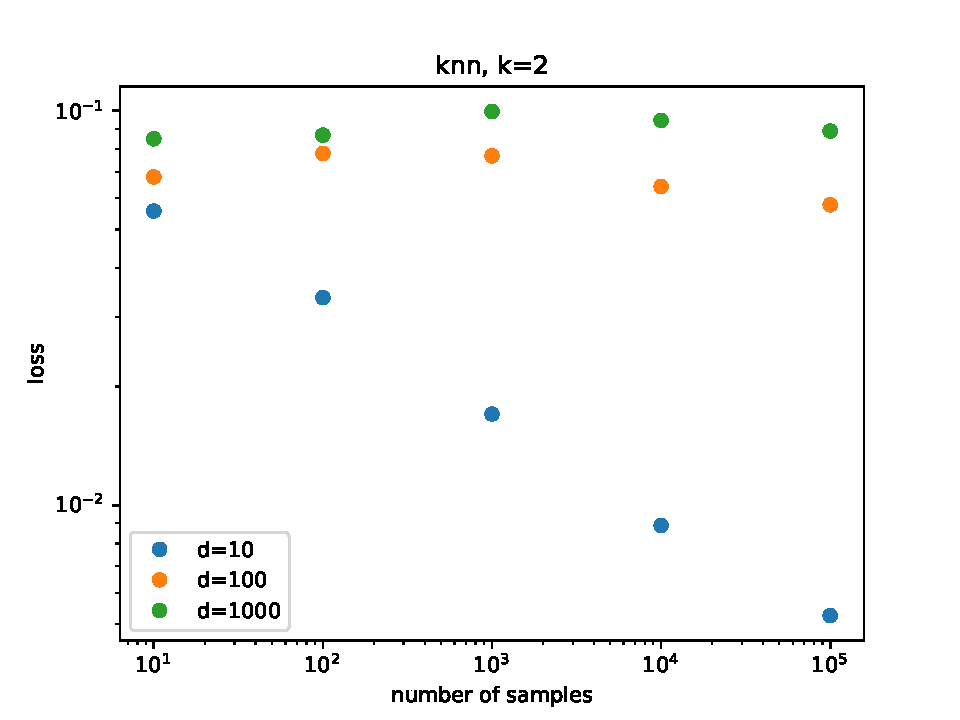
\includegraphics[width=0.8\linewidth]{knnd}
        \label{fig:knnd}
    \end{figure}
    
\end{frame}



\subsection{Optimization}%
\label{sub:optimization}

    \begin{frame}{Optimization}

	As we will discuss shortly, learning is reformulated as an \textbf{optimization problem}. We often have to optimize functions that are \textbf{{hard}} to
        optimize.

        \begin{itemize}
            \item non convexity
            \item non linearity
	    \item high dimension
            \item instability of estimators
        \end{itemize}
    \end{frame}

    \begin{frame}{Convex function}
	\begin{figure}[htpb]
		\centering
		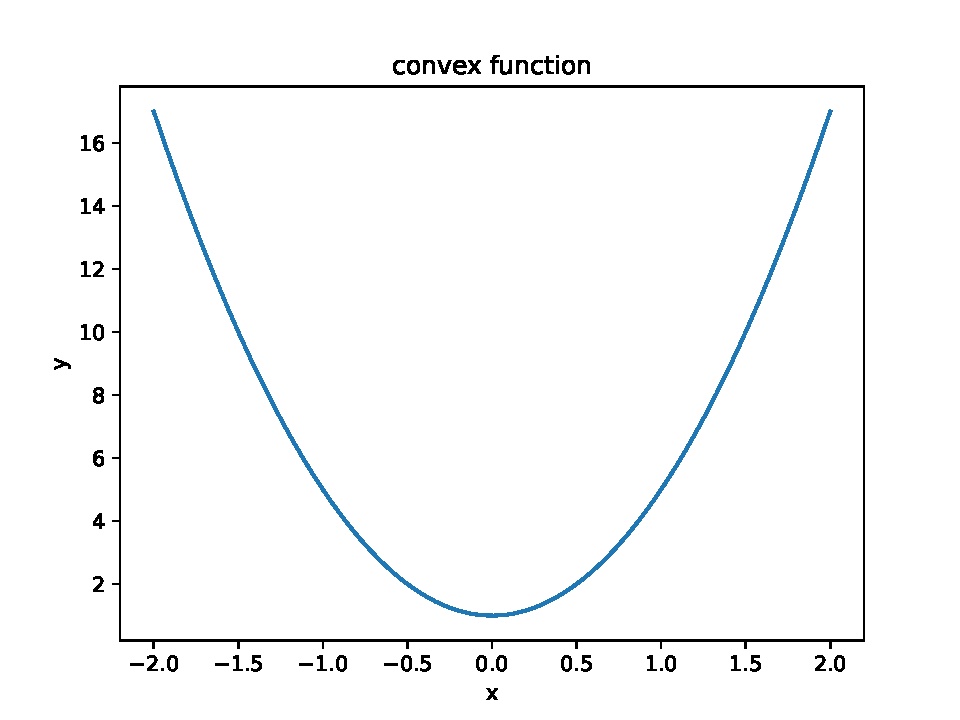
\includegraphics[width=0.8\textwidth]{convex}
		\label{fig:convex}
	\end{figure}
    \end{frame}

    \begin{frame}{Non-convex function}
	\begin{figure}[htpb]
		\centering
		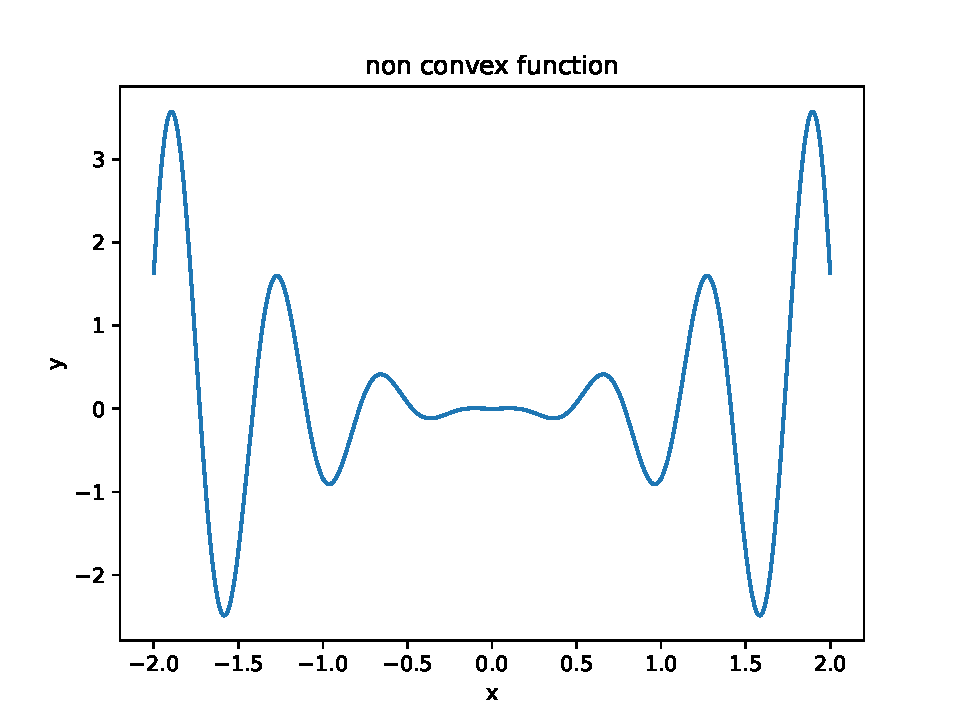
\includegraphics[width=0.8\textwidth]{nonconvex}
		\label{fig:convex}
	\end{figure}
    \end{frame}


\begin{frame}{The state of ML}
    ML is an active research area. One of the biggest effort is trying to understand the performance of deep learning.
    \begin{itemize}
        \item they are non convex
	\item but we experimentally manage to optimize them so that they have a state-of-the-art generalization error
    \end{itemize}
    In the case of neural networks with $1$ hidden layer, the convergence of gradient descent to a global minimizer of the objective function has been proven in 2018 in a specific case (large number of hidden neurons), using tools from optimal transport theory (\cite{chizat2018global}).
\end{frame}

\begin{frame}{The double descent phenomenon (we will discuss it again later)}
    \begin{figure}[htpb]
        \centering
        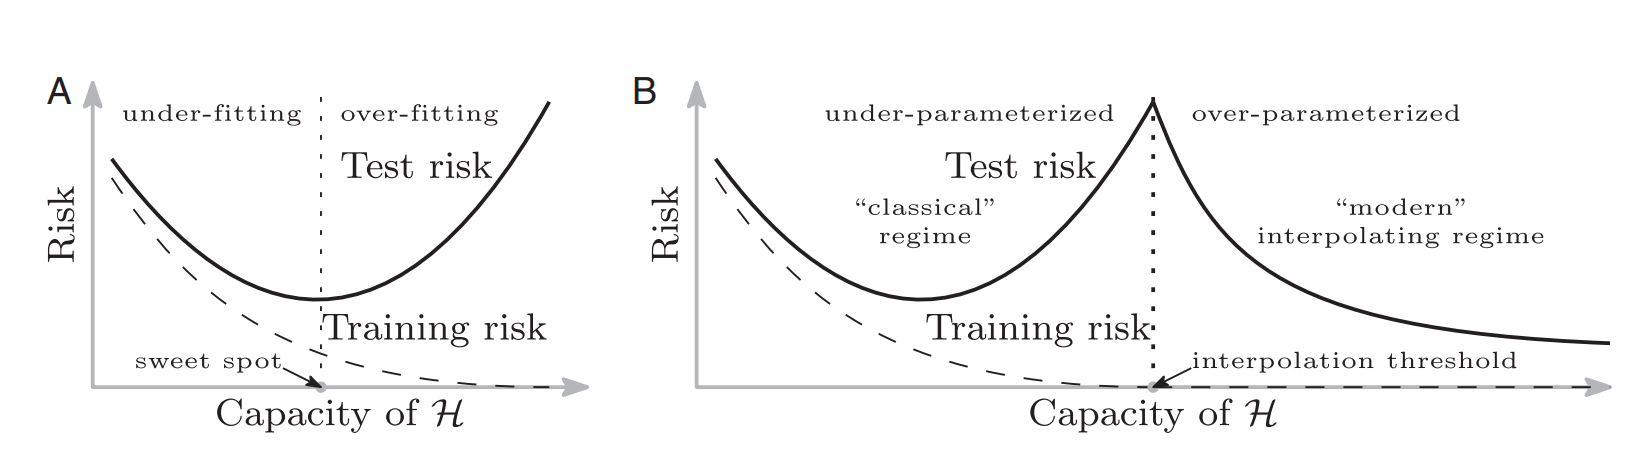
\includegraphics[width=1\textwidth]{doubledescent}
	\caption{[Belkin et al, 2019]}
        \label{fig:}
    \end{figure}
\end{frame}


\begin{frame}[allowframebreaks]
\frametitle{References}
\bibliographystyle{apalike}
\bibliography{epitech.bib} 
\end{frame}

\end{document} 
